\documentclass[a4paper,twoside,onecolumn]{report}
\author{Bartosz Grabski}
\title{Narzędzia informatyki}
\date{\today}

\usepackage{graphicx}
\usepackage[polish]{babel}
\usepackage[OT4]{fontenc}
\usepackage[utf8]{inputenc}

\usepackage{tabularx}
\usepackage{amsmath}
\usepackage{amssymb}
\usepackage{amsfonts}

\usepackage{epigraph}
\usepackage{enumerate}

 \begin{document}
 	\maketitle

	\section{Wstęp}
		\epigraph{
			Nie godzi się aby zdolni ludzie tracili godziny, jak niewolnicy, wykonując obliczenia, gdy taką pracę można przekazać bezpiecznie komukolwiek korzystającemu z maszyn
		}{
			\textit{Gottfried Wilhelm von Leibniz 
		}}
	
	\section{Historia}
		\begin{enumerate}[-]
			\item Prehistoria
				\begin{enumerate}[*]
					\item 1820 - Charles Xavier Thomas de Colmar - arytmometr - pierwszy masowo produkowany mechaniczny kalkulator
					\item 1801 - Joseph-Marie Jacquard - maszyny dziewiarskie programowane za pomocą kart dziurkowanych
					\item 1837 - Charles Babbage - w 1837 r. opisał projekt maszyny analitycznej Maszyna programowana za pomocą kart dziurkowanych i napędzana parą 								Problemy z precyzją wykonania spowodowały porzucenie projektu zbudowania maszyny
					\item 1843 - Ada Lovelace przetłumaczyła artykuł Luigi Menabrea o maszynie analitycznej i dodała swój komentarz, m.in. program obliczania sekwencji liczb 								Bernouliego
					\item 2002 - zbudowano maszynę różnicową w Londynie: 4000 elementów, 3 tony, 3x1.8 m
					\item Pod koniec lat 80-tych XIX w. Herman Hollerith opracował system zapisu i przetwarzania danych oparty na kartach dziurkowanych
					\item Opracował tabulator i maszynę dziurkującą
					\item 1890 - spis powszechny w USA wykorzystał w/w technologie
					\item 1896 założył Tabulating Machine Company
					\item 1911 połączył się z 3 innymi firmami tworząc Computing Tabulating Recording Company
					\item 1924 firma zmieniłą nazwę na International Business Machines
				\end{enumerate}
			\item Kalkulatory
				\begin{enumerate}[*]
					\item Kalkulatory mechaniczne
					\item W 1948 Curt Herzstark opracował ręczny kalkulator Curta Pierwszy model kosztował $125 (dzisiaj $1596) Zastąpiły go dopiero kalkulatory elektroniczne
				\end{enumerate}
			\item Rozwój elektroniki
				\begin{enumerate}[*]
					\item 1904 - John Anbrose Fleming - Dioda próżniowa
					\item 1906 - Lee De Forest - Trioda próżniowa
					\item 1947 - Tranzystor - John Bardeen, Walter H. Brattain, W. Shockley (Bell) (Nagroda Nobla 1956 r.)
					\item 1958 - Układy scalone - Jack Kilby TI (Nagroda Nobla 2000 r.)
				\end{enumerate}
			\item Rozwój układów scalonych
				\begin{enumerate}[*]
					\item 1971 - Intel 4004 - 2.250 tranzystorów, 10000nm
					\item 1978 - Intel 8086 - 2.9000 tranzystorów, 3000nm
					\item 1993 - Intel Pentium - 3.100.100 tranzystorów. 800nm
					\item 2022 - Apple A16 - 16.000.000.000 tranzystorów, 4nm
				\end{enumerate}
			\item Urządzenia
				\begin{enumerate}[*]
					\item 1962 - Pierwszy kalkulator elektroniczny - ANITA Mk. VII - 1962 Zbudowany na lampach (177) Wyświetlacz z lamp Nixie Cena ok. 350 GBP Produkowane 						w różnych odmianach do połowy lat 70-tych
					\item 1963 - Pierwszy kalkulator tranzystorowy - Friden EC-130 - 13 cyfrowa dokładność wyświetlacz kineskopowy obliczenia w logice RPN cena \$2200 (dzisiaj 							\$22128)
				\end{enumerate}
			\item Komputery analogowe
				\begin{enumerate}[*]
					\item Konstrukcja komputera związana z rozwiązywanym problemem Najróżniejsze modele: oparte na prądzie, na przepływie cieczy, pneumatyczne Np. 								komputer sterowania ogniem wykorzystywany przez US Navy
				\end{enumerate}
			\item Alan Turing
				\begin{enumerate}[*]
					\item 1936 - opublikował pracę „ON COMPUTABLE NUMBERS, WITH AN APPLICATION TO THE ENTSCHEIDUNGSPROBLEM” Opisał w nim problem stopu A co 							ważniejsze model maszyny obliczeniowej nazywanej teraz maszyną Turinga
					\item 1945 - W oparciu o maszynę Turinga w 1945 r. John von Neumann zaproponował uniwersalną architekturę komputera Dane i program traktowane są w 							ten sam sposób Prawie każdy współczesny komputer realizuje architekturę von Neumanna
				\end{enumerate}
			\item Komputery
				\begin{enumerate}[*]
					\item 1936 - Konrad Zuse rozpoczął w Niemczech prace nad programowanym kalkulatorem - model Z1 
					\item 1941 - powstał komputer Z3 Wykorzystywał logikę binarną, liczby zmiennoprzecinkowe Dane zapisywane na dziurkowanym filmie 35 mm Po wojnie Zuse 						opracował język wysokiego poziomu Plankalkül zaimplementowany w 2000 r. IBM przejął jego patenty w zamian za finansowanie działalności
					\item 1941-1944 - Colossus - komputer zbudowany do łamania kodów niemieckich przez anglików Skonstruowany w latach 1941-44 W sumie 10 sztuk Mało 								uniwersalny, programowany za pomocą przełączników, dane z taśmy perforowanej Po wojnie zniszczony i utajniony do 1970 r.
					\item 1937 - Claude Shannon (MIT) udowodnił w doktoracie, że istnieje bezpośrednie przełożenie logiki boolowskiej na bramki logiczne
					\item 1938 - George Stiblitz (Bell) zbudował komputer na bramkach „Model-K” 
					\item 1940 - zbudowali Complex Number Calculator wykonujący obliczenia na liczbach zespolonych Pierwszy komputer umożliwiający pracę zdalną przez linię 								telefoniczną
					\item 1939 - rozpoczęły się prace nad Harvard Mark I sponsorowane przez IBM Bardzo skomplikowana konstrukcja, napędzana silnikiem spalinowym 800 km 								przewodów, 3 miliony połączeń Pamięć na 72 23-cyfrowe liczby 3 dodawania/odejmowania na sekundę mnożenie 6 sekund, dzielenie 15 sekund Brak 								instrukcji rozgałęziających i pętli
					\item 1943-46 - Electronic Numerical Integrator and Computer Zbudowany do obliczenia tablic artyleryjskich Pierwszy w pełni cyfrowy komputer uniwersalny
						Zbudowany w latach 1943-46 Po przeprowadzce działał bez przerwy od 1947 do 1955 r. 17468 lamp, 7200 diod, 1500 obwodów, 70000 oporników, 								10000 kondensatorów, 5 mln punktów lutowania 167 m2, 2.4 x 0.9 x 30 m, 27 ton 357 operacji dodawania na sekundę, 35 dzielenia
					\item 1948 - Manchester Small-Scale Experimental Machine Eksperymentalny komputer wyposażony w pamięć Uruchomiony w 1948 r. Stał się podstawą 								pierwszego komercyjnego komputera Ferranti Mark 1
					\item EDVAC (Electronic Discrete Variable Automatic Computer) - następca ENIAC
					\item EDSAC (Electronic Delay Storage Automatic Calculator) - komputer angielski 1949 r.
					\item MECM - pierwszy komputer radziecki 1950 r. (6 tys lamp, 24 kW mocy)
					\item CSIRAC (Council for Scientific and Industrial Research Automatic Computer) - Australia 1949 r.
				\end{enumerate}
			\item Komputery
				\begin{enumerate}[*]
					\item lampy Williamsa - rodzaj miniaturowego kineskopu
				\end{enumerate}
			\item Komputery komercyjne
				\begin{enumerate}[*]
					\item Ferranti Mark 1 - 1951 r.
					\item LEO 1 - 1951 r.
					\item UNIVAC1 (Universal Automatic Computer) - 1951 r. pamięć na taśmie magnetycznej
					\item IBM 701 - 1954 r.
					\item FORTRAN dla IBM 704 - 1956 r.
					\item IBM 350 RAMAC (Random Access Method of Accounting and Control) - pierwszy dysk twardy - 1956 r., 5 MB - $50000 (dzisiaj $565788)
				\end{enumerate}
			\item Komputery polskie
				\begin{enumerate}[*]
					\item Komputery polskie
					\item Odra 1001 - prototyp lampowy z 1961 r.
					\item Odra 1002 - prototyp lampowo-tranzystorowy z 1962 r.
					\item Odra 1003 - komputer tranzystorowy z lat 1963-65 - 42szt.
					\item Odra 1013 - tranzystorowy, pamięć ferrytowa, 1966-67, 84 szt.
					\item Odra 1103 - tranzystorowy, 1967-1969, 64 szt. 
					\item Odra 1204 - komputer mikroprogramowalny, 1967-1972, 179 szt.
				\end{enumerate}
			\item Komputery polskie Komputery na licencji International Computers Limited:
				\begin{enumerate}[*]
					\item Odra 1304 - 1970-73, 90 szt.
					\item Odra 1305 - od 1973 r., 346 szt., ostatnia wyłączona w 2010 r.
					\item Odra 1325 - od 1973 r., układy scalone, 151 szt. 
					\item języki Fortran, Cobol, Algol, ...
				\end{enumerate}
			\item Komputery tranzystorowe
				\begin{enumerate}[*]
					\item Tranzystor - 1947 r. University of Manchester 1953 r.
					\item 1955 r. - 200 tranzystorów, 1300 diod, 150W
					\item Hardwell Cadet 1955 r. MTBF - 90 minut 
					\item IBM 1401 - 1959 r. - 10 tys. sztuk
					\item PDP-1 - Digital Equipment Corporation - 1959 r
				\end{enumerate}
			\item Układy scalone
				\begin{enumerate}[*]
					\item Powstanie mikroprocesora i układów pamięci
					\item Minikomputery
					\item Olivetti P6060
					\item MOS Technology KIM1
					\item Altair 8800
				\end{enumerate}
			\item Altair 8800
				\begin{enumerate}[*]
					\item Zestaw do samodzielnego montażu (\$440) lub
					\item zmontowany (\$620)
					\item Intel 8080
					\item Możliwość pracy z 8” stacją dyskietek
					\item Firma planowała sprzedaż na kilkaset sztuk łącznie, w ciągu miesiąca sprzedali ponad 1 tys. Altair Basic
				\end{enumerate}
			\item Apple
				\begin{enumerate}[*]
					\item Apple I - 1976 r. - pierwszy hobbystyczny komputer sprzedawany jako płyta główna, Trzeba było dokupić zasilacz i klawiaturę oraz mieć monitor Cena 								\$666,66 (po uwzględnieniu inflacji na 2023 rok - \$3,602)
					\item Wyprodukowano 200 szt., szacuje się, że dzisiaj istnieje >=62 szt.
					\item Apple II - 1977 r. W pełni złożony komputer z kolorową grafiką Cena \$1298 (na dzisiaj \$6,592) Sprzedano 4.8 mln szt. 
					\item 1984 - Macintosh - pierwszy komputer komercyjne dostępny z okienkowym systemem operacyjnym \$2495 (na dzisiaj \$7,391)
				\end{enumerate}
			\item IBM PC
				\begin{enumerate}[*]
					\item IBM 5150 - 12.08.1981 r. \$1565 bez napędów (na dzisiaj \$5,299) Projekt ogólnodostępny z wyjątkiem BIOS Intel 8088 - prostsza wersja 8086
				\end{enumerate}
			\item Mikrokomputery 8-bitowe
				\begin{enumerate}[*]
					\item Commodore PET - 1977 r., MOS 6502
					\item Atari 400 i 800 - 1979 r., MOS 6502
					\item ZX Spectrum, 1982 r., Zilog Z80
					\item Commodore 64, MOS 6502
				\end{enumerate}
			\item Mikrokomputer polski
				\begin{enumerate}[*]
					\item Elwro 800 Junior - 1986 r.
					\item Opracowany przez PP i Elwro
					\item Obudowa po organkach Elwirka
					\item Kompatybilny z ZX Spectrum
					\item Sieciowy system CP/J odmiana CP/M
					\item Kompilator Borland Turbo Pascal 3.0
				\end{enumerate}
			\item Palmtopy
				\begin{enumerate}[*]
					\item Palm Pilot 1000 - 1996 r., Palm OS 1.0
					\item HP Jornada 420 - 1999 r., Windows CE 2.11
					\item Handspring Treo 180 - 2002 r., Palm OS 3.5,
					\item telefon GSM
					\item HP Jornada 928 - 2002 r, Pocket PC 2002,
					\item telefon GSM, GPRS
				\end{enumerate}
			\item Smartfony
				\begin{enumerate}[*]
					\item Nokia 9210 Communicator, 2000 r., Symbian Series 80
					\item Nokia 7650 - 2002 r., Symbian Series 60
					\item Sony Ericsson P800 - 2002 r., Symbian UIQ
					\item BlackBerry 6230 - 2003 r.,
					\item iPhone - 2007 r., iPhone OS 1.0
					\item HTC T1 - 2007 r., Android
				\end{enumerate}
			\item Tablety
				\begin{enumerate}[*]
					\item Apple iPad - 2010 r., iOS 3
					\item Tablety z Androidem
					\item Czytniki eBook i inne
					\item dedykowane urządzenia
				\end{enumerate}
			\item Przyszłość
				\begin{enumerate}[*]
					\item Komputery kwantowe
					\item „Rozszerzone” okulary
					\item Dalszy rozwój „wearables”
					\item Interfejsy neuronalne
				\end{enumerate}
		\end{enumerate}
	\section{Latex}
		\begin{enumerate}
			\item Dlaczego nie WORD
			\begin{enumerate}
				\item Różne wersje programu (także językowe i systemowe)
				\item Jest edytor równań, ale może się różnić między wersjami
				\item Dokument wyjściowy może zależeć od skonfigurowanej w systemie drukarki
				\item Kwestia różnych ,,czcionek''
				\item Niska ,,stabilność'' dokumentu
			\end{enumerate}

			\item CZYM JEST TEX?
			\begin{enumerate}
				\item System składu tekstu niskiego poziomu
				\item Opracowany pierwotnie w latach 1977/78 przez Donalda Knuth’a ze Stanford
				\item Był niezadowolony ze składu drugiej edycji swojej książki The Art of Computer Programming
				\item Postanowił to zmienić i zaczął tworzyć własne narzędzie na platformie PDP-10
				\item System dostępny na zasadzie Open Source
				\item Wszystkie błędy zostaną uznane za cechy
				\item System ma być stabilny, aby dokumenty stworzone kiedyś w przyszłości wyglądały tak samo
			\end{enumerate}

			\item CZYM JEST LATEX?
			\begin{enumerate}
				\item Zestaw makr rozbudowujących funkcjonalność TEX’a
				\item Opracowany przez Lesliego Lamporta ze Stanford na początku lat 80-tych
				\item Wydana w 1986 książka LaTeX User Manual
				\item Aktualnie wersja LaTeX 2E (prace nad wersją 3 zostały wstrzymane)
				\item Również dostępny jako Open Source
				\item (La)TeX to w praktyce język programowania, którego wynikiem jest dokument
				\item Nie jest narzędziem WYSIWYG (What You See Is What You Get) jak np. Microsoft Word
				\item Jest dostępny na wielu systemach operacyjnych
				\item Wiele różnych dystrybucji
			\end{enumerate}

			\item PRZYKŁADOWE DYSTRYBUCJE
			\begin{enumerate}
				\item MiKTeX - www.miktex.org Windows, macOS, Linux, Dołączony menedżer pakietów
				\item TeXLive - www.tug.org/texlive Windows, Linux 
				\item MacTeX - www.tug.org/mactex, Wersja TeXLive dla macOS
				\item WERSJA ONLINE Środowisko Overleaf - overleaf.com Praca on-line Repozytorium dokumentów Wersja darmowa z ograniczeniami Wersje płatne
			\end{enumerate}

			\item PLIK LATEX
			\begin{enumerate}
				\item Zwykły plik tekstowy ASCII (najlepiej UTF-8) zawierający:
				\item Polecenia (instrukcje) LaTeX’a,
				\item Treść dokumentu,
				\item Inne symbole sterujące.
				\item Można edytować w dowolnym edytorze, np. Notatniku
			\end{enumerate}

			\item ODSTĘPY
			\begin{enumerate}
				\item Liczba spacji między wyrazami nie ma znaczenia.
				\item Pusty wiersz rozpoczyna nowy akapit
			\end{enumerate}

			\item ZNAKI SPECJALNE
			\begin{enumerate}
				\item Ich użycie jest zarezerwowane
				\item Mają specjalne znaczenie
				\item Jak chcemy ich użyć w tekście poprzedzamy je
				\item Nie są dostępne we wszystkich krojach pisma 
			\end{enumerate}

			\item POLECENIA (INSTRUKCJE)
			\begin{enumerate}
				\item Instrukcje zaczynają się od \\ bezpośrednio po którym jest nazwa
				\item Instrukcję kończy spacja (odstęp) lub znak niebędący literą
				\item Składnia instrukcja jest wrażliwa na wielkość liter
				\item Niektóre instrukcję składają się z \\ i jednego znaku niebędącego literą
				\item Niektóre instrukcje mają argumenty:
				\item Podawane w nawiasach klamrowych \{ \}
				\item Każdy w osobnej parze nawiasów
				\item Liczba oraz kolejność argumentów jest istotna
				\item Instrukcje mogą mieć argumenty opcjonalne w nawiasach kwadratowych [ ]
				\item Argumenty opcjonalne rozdziela się przecinkami,
				\item Kolejność nie odgrywa roli
				\item Komentarz po znaku % do końca linii
			\end{enumerate}

			\item STRUKTURA DOKUMENTU
			\begin{enumerate}
				\item Preambuła - Tu definiujemy typ dokumentu i wykorzystywane pakiety
				\item Część główna - Tu znajduje się treść dokumentu
			\end{enumerate}

			\item PREAMBUŁA
			\begin{enumerate}
				\item Obowiązkowo \textbackslash documentclass\{article\}
				\item Przykładowe typy: article, report, book, slides, letter
				\item Opcjonalnie w kolejnych liniach, np.  \textbackslash usepackage\{graphicx\}
				\item Przykład:\\
					\textbackslash documentclass[a4paper,twoside,onecolumn]\{report\} \\
					\textbackslash usepackage{graphicx} \\
					\textbackslash author\{Bartosz Grabski\} \\
					\textbackslash title\{Narzędzia informatyki\} \\
					\textbackslash date\{\textbackslash today\} \\
			\end{enumerate}

			\item CZĘŚĆ GŁÓWNA
			\begin{enumerate}
				\item Wszystko pomiędzy: \textbackslash begin\{document\} . . . \textbackslash end\{document\}
			\end{enumerate}

			\item STRUKTURA DOKUMENTU
			\begin{enumerate}
				\item Dokument może być podzielony na sekcje, czyli rozdziały, podrozdziały, itd. \{document\} \\
					\textbackslash begin\{document\}
						Początkowe zdanie \\
						\textbackslash section\{Wstęp\} \\
						Treść wstępu \\
						\textbackslash section\{Sekcja głowna\} \\
						Treść sekcji głownej \\
						\textbackslash subsection\{Podpunkt pierwszy\} \\
						Treść podpunktu pierwszego \\
						\textbackslash subsubsection\{Podpodpunkt pierwszy\} \\
						Treść podpodpunktu pierwszego \\
						\textbackslash end\{document\}
			\end{enumerate}


			\item TYTUŁ DOKUMENTU
			\begin{enumerate}[*]
				\item W niektórych typach dokumentów (np. article, book) można automatycznie wygenerować tytuł
				\item Definiowany jest w preambule\\
					\textbackslash author\{Bartosz Grabski\} \\ 
					\textbackslash title\{Narzędzia informatyki\} \\
					\textbackslash date\{\textbackslash today\} \\
					\textbackslash begin\{document\} \\
					\textbackslash maketitle \\
					\textbackslash end\{document\} \\
				\item Polecenia date może zawierać:
				\item Datę dzisiejszą - \textbackslash today
				\item Dowolny tekst
				\item Być puste wtedy daty nie będzie w dokumencie
			\end{enumerate}

			\item STEROWANIE CZCIONKAMI
			\begin{enumerate}[*]
				\item Wyróznienie - \textbackslash emph\{słowo\} - \emph{słowo}
				\item Krój maszynowy - \textbackslash texttt \{słowo\} - \texttt{słowo}
				\item Krój bezszeryfowy - \textbackslash textsf \{słowo\} - \textsf{słowo}
				\item Krój szeryfowy - \textbackslash sf \{słowo\} - \sf{słowo}
				\item małe - \textbackslash small \{słowo\} - \small{słowo}
				\item duże - \textbackslash large \{słowo\} - \large{słowo}
				\item kursywa - \textbackslash textit \{słowo\} - \textit{słowo}
				\item pogrubiony - \textbackslash textbf \{słowo\} - \textbf{słowo}
			\end{enumerate}

			\item ŁAMANIE LINII
			\begin{enumerate}[*]
				\item \textbackslash noindent - likwiduje wcięcie na na początku akapitu
				\item Niełamliwa spacja - tylda
				\item \textbackslash newpage - nowa strona
				\item \textbackslash pagebreak[liczba]
				\item \textbackslash textbackslash nowy akapit
				\item \textbackslash textbackslash \* nowa linia ale nie akapit
				\item \textbackslash nolinebreak
				\item \textbackslash nopagebreak
			\end{enumerate}

			\item ODSTĘPY
			\begin{enumerate}[*]
				\item \textbackslash hspace\{3cm\} - odstęp poziomy
				\item \textbackslash vspace\{3cm\} - odstęp pionowy
				\item \textbackslash vspace\{3cm\} - odstęp pionowy
				\item \textbackslash stretch\{3cm\} - wypełnienie w hspace
				\item \textbackslash hfill - wypełnienie
			\end{enumerate}

			\item ZNAKI SPECJALNE
			\begin{itemize}
				\item CUDZYSŁOWY - startowy: 2 przecinki, końcowy: 2 apostrofy
				\item MYŚLNIKI
				\begin{itemize}
					\item łącznik - 22-go
					\item pauza -- 2x minus
					\item myślnik - zwykły --- 3x minus
				\end{itemize}
			\end{itemize}

			\item ŚRODOWISKA
			\begin{itemize}
				\item Sekcja zawarta pomiędzy begin a end
				\item Mogą się nawzajem zawierać ale nie przeplatać
				\item Używane do tworzenia list, tabel i innych złożonych konstrukcji
			\end{itemize}

			\item LISTY \\
			\begin{itemize}
				\item przykład
					\textbackslash begin\{enumerate\} \\
					\textbackslash item Pierwszy punkt listy z numerami \\
					\textbackslash begin\{itemize\} \\
					\textbackslash item Lista bez numerków \\
					\textbackslash end\{itemize\} \\
					\textbackslash begin\{description\} \\
					\textbackslash item [Tytuł] jakiś tam opis \\ 
					\textbackslash end\{description\} \\
					\textbackslash begin\{enumerate\} \\
				\item pakiet enumerate - umożiwia nadawania wartości początkowej liście wyliczeniowej
			\end{itemize}

			\item WYRÓWNANIE TEKSTU
			\begin{itemize}
				\item Środowiska flushleft, flushright i center
			\end{itemize}


			\item TABELE
			\begin{itemize}
				\item Środowisko tabular
				\item Po otwarciu podajemy sposób wyrównywania każdej kolumny (rac, l) oddzielony ewentualnie pionową kreską
				\item Komórki oddzielamy \& a wiersze \textbackslash \textbackslash
				\item \textbackslash hline rysuje poziomą linię 
				\item Łączenie komórek i inne linie \textbackslash multicolumn
				\item Przykład \\
					\begin{tabular}{|c|c|c|c|l|}
						\hline
						1 & 2 & 3 & 4 & 5 \\
						\cline{2-5}
						1 & \multicolumn{3}{|r|}{ddd} & 5 \\
						\cline{2-5}
						1 & 2 & 3 & 4 & 5 \\
						\hline
					\end{tabular}
				\item lina pozioma - \textbackslash hline - przez całość
				\item lina pozioma - \textbackslash cline\{2-3\} - od-do
				\item definicja justowania - \textbackslash begin\{tabular\}\{|c|c|c|c|l|\}
			\end{itemize}

			\item ODSYŁACZE - odsyłanie do elementów struktury dokumentu
			\begin{itemize}
				\item \textbackslash ldots - trzykropki
				\item \textbackslash label - kotwica odsyłacza
				\item \textbackslash ref - użycie odsyłacza
			\end{itemize}

			\item WSTAWKI
			\begin{itemize}
				\item Zazwyczaj chcemy aby tabele czy rysunki nie były dzielone pomiędzy stronami, były podpisane i można się było do nich odwoływać
				\item Służą do tego środowiska table i figure
				\item Oba mają pewne parametry ustalające miejsce, w którym znajdzie się wstawiony element (por. dokumentacja)
				\item \textbackslash caption{wyświetlana nazwa} - \textbackslash label{kotwica}
				\item środowisko table \\
					\textbackslash begin\{table\}\\
						\textbackslash begin\{tabular\}\\
						\textbackslash end\{tabular\}\\
						\textbackslash caption\{wyświetlana nazwa\} \textbackslash label\{kotwica\}\\
					\textbackslash end\{table\}\\
					Wstawienie: \{ \textbackslash \tt table\}
			\end{itemize}

			\item OBRAZKI\\
				\textbackslash begin\{figure\}\\
					\textbackslash centering \\
					\textbackslash includegraphics[width=8cm]\{fig1.png\}\\
					\textbackslash caption\{wyświetlana nazwa\}
				\textbackslash end\{figure\}\\

			\item MATEMATYKA
			\begin{itemize}
				\item Do pisania wzorów wykorzystujemy znak specjalny \$
				\item Funkcje matematyczne mają odpowiadające im polecenia
				\item Równanie można umieścić w osobnej linii dzięki \textbackslash [ i \textbackslash ] lub \$\$ \ldots \$\$
				\item Możemy skorzystać ze środowiska equation, które pozwala na etykietowanie wzorów
				\item Można się potem do nich odwoływać
				\item W środowisku equation nie używamy \$
				\item Jeżeli nie chcemy numerować wzoru to po equation dodajemy * - begin\{equation*\}
				\item Sposoby tworzenia równań można do pewnego stopnia mieszać
				\item \_  - index dolny
				\item \^ - index górny
				\item \textbackslash frac\{licznik\}\{mianownik\} - ułamek
				\item \textbackslash sum - sigma, znak sumy
				\item \textbackslash circ - znak stopnia, trzeba umieścić w indexie górnym
				\item niestandardowe odstępy \\
					\begin{tabular}{ccc}\\
						\textbf{Skrót}      & \textbf{Polecenie}              & \textbf{Przykład} \\
						\textbackslash ,    & \textbackslash thinspace     & a \, b \, c \\
						\textbackslash :  & \textbackslash medspace    & a \: b \: c \\
						\textbackslash ;  & \textbackslash thickspace    & a \; b \; c \\
						brak  & \textbackslash quad    & a \quad b \quad c \\
						brak  & \textbackslash qquad    & a \qquad b \qquad c \\
						\textbackslash !  & \textbackslash negthtinspace    & a \negthinspace b \negthinspace c \\
						brak  & \textbackslash negmedspace    & a \negmedspace b \negmedspace c \\
						brak  & \textbackslash negthickspace    & a \negthickspace b \negthickspace c \\
					\end{tabular}
				\item Jeżeli chcemy umieścić w równaniu fragment tekstu to służy do tego polecenie \textbackslash text\{Litery greckie\}
				\item Nasze możliwości tworzenia równań wzrosną, gdy użyjemy pakietów \emph{amssymb} i \emph{amsmath} opracowanym przez Amerykańskie Stowarzyszenie 							Matematyków (AMS) 
			\end{itemize}

			\item Rozmieszczanie równań
			\begin{itemize}
				\item \textbackslash begin\{split\} - formatowanie jak w tabeli
				\item \textbackslash begin\{multiline\} - wyśrodkowane linijkami
				\item \textbackslash begin\{gather\} - wyśrodkowane w kolumnach
				\item \textbackslash begin\{align\} - do lewej
			\end{itemize}

			\item Warunki
			\begin{itemize}
				\item \textbackslash begin\{cases\} - formatowanie jak w tabeli
			\end{itemize}

			\item Macierze
			\begin{itemize}
				\item \textbackslash begin\{matrix\} - formatowanie jak w tabeli, bez nawiasów
				\item \textbackslash begin\{pmatrix\} - formatowanie jak w tabeli, nawiasy okrągłe
				\item \textbackslash begin\{vmatrix\} - formatowanie jak w tabeli, nawiasy proste
				\item \textbackslash begin\{Vmatrix\} - formatowanie jak w tabeli, nawiasy proste podwójne
				\item \textbackslash begin\{bmatrix\} - formatowanie jak w tabeli, nawiasy kwadratowe
			\end{itemize}

			\item Macierze - środowisko array
			\begin{itemize}
				\item \textbackslash begin\{array\}{cc} - formatowanie jak w tabeli, nawiasy okrągłe
			\end{itemize}

			\item BIBLIOGRAFIA
			\begin{itemize}
				\item LaTeX wspomaga tworzenie bibliografii, zarządzanie nią i tworzenie odnośników
				\item Przy pierwszej kompilacji dokumentu tworzony jest pliku pomocniczy aux
				\item Dopiero przy drugiej kompilacji odnośniki będą poprawne
				\item W najprostszym przypadku umieszczamy w dokumencie środowisko thebibliography
				\item Poszczególne pozycje są umieszczane w poleceniu \textbackslash bibitem
				\item Cytowanie w tekście poprzez \textbackslash cite
				\item Do zarządzania cytowaniami można wykorzystać narzędzie BibTeX lub BibLaTeX
				\item Spis literatury jest wtedy przechowywany w osobnym pliku
				\item Do dokumentu trafi lista tylko wykorzystanych pozycji
			\end{itemize}

		\end{enumerate}


	\begin{figure}[h]
		\centering
		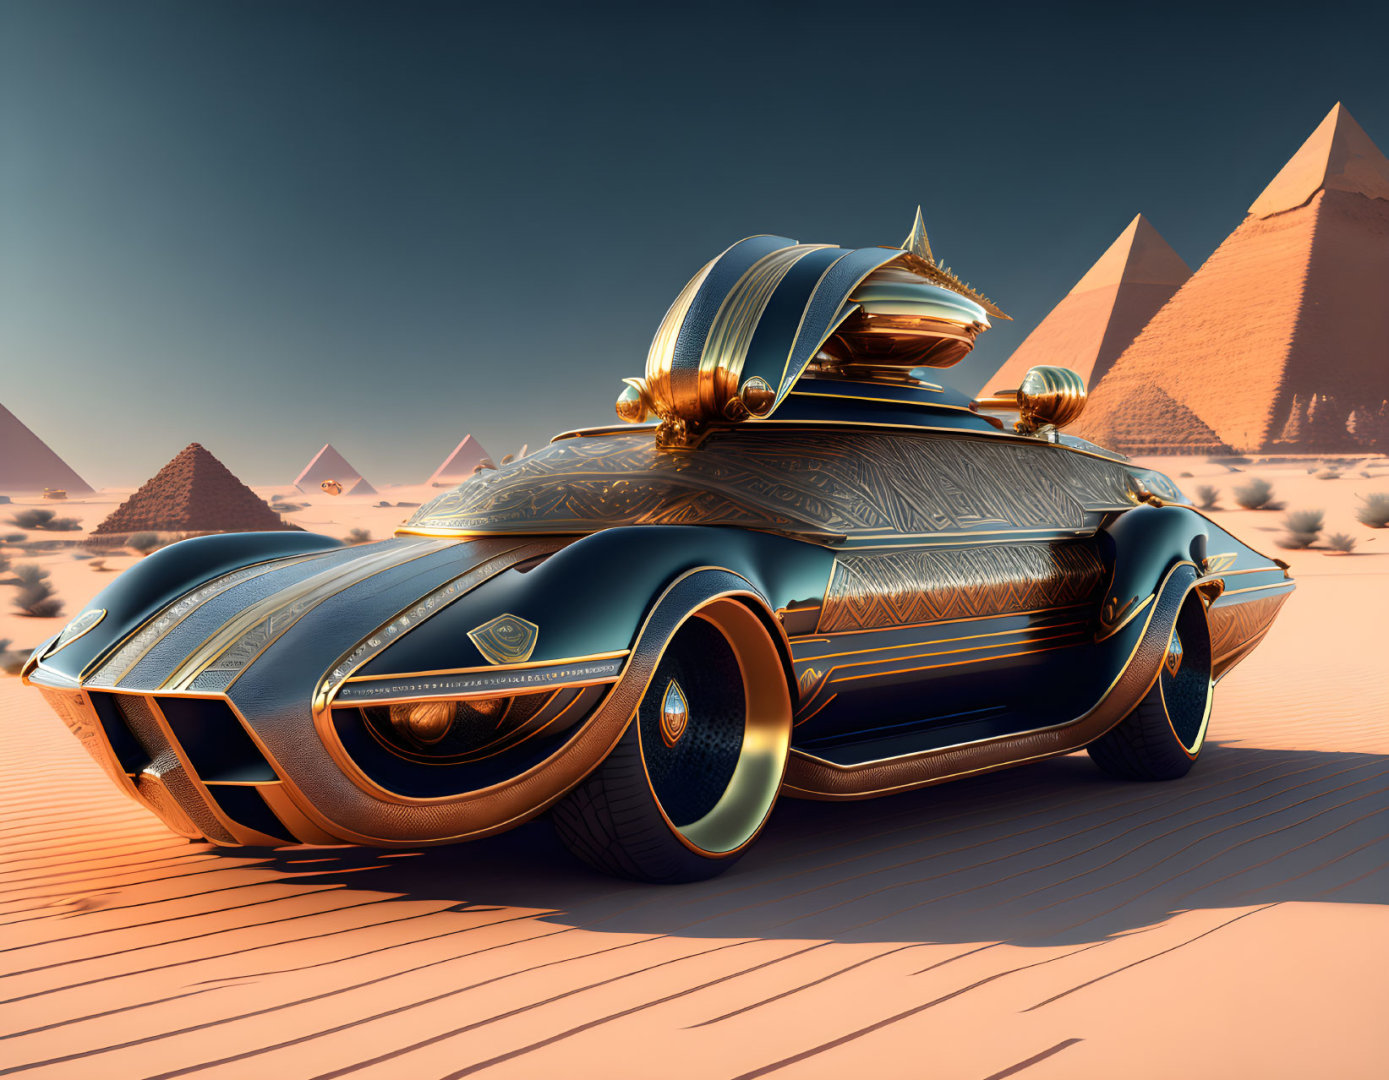
\includegraphics[width=0.5\textwidth]{picture1.jpg}
		\caption{Basic principle of tomography.}
	\end{figure}

\end{document}